% IEEE Paper Template for US-LETTER Page Size (V1)
% Sample Conference Paper using IEEE LaTeX style file for US-LETTER pagesize.
% Copyright (C) 2006-2008 Causal Productions Pty Ltd.
% Permission is granted to distribute and revise this file provided that
% this header remains intact.
%
% REVISION HISTORY
% 20080211 changed some space characters in the title-author block
%
\documentclass[10pt,conference,letterpaper]{IEEEtran}
\usepackage{times}
\usepackage{amsmath}
\usepackage{graphicx}
\usepackage[caption=false,font=footnotesize]{subfig}
\usepackage{booktabs}
\usepackage{multirow}
\usepackage{tabularx}
\usepackage{tabu}
\usepackage{amsthm}
\usepackage{bm}
\usepackage{xspace}
\usepackage{pgfplots}
\usepackage{enumerate}
\usepackage[ruled]{algorithm2e}
\usepackage{balance}
\usepackage{chronosys, txfonts}
%\usepackage[keeplastbox]{flushend}
\graphicspath{ {images/} }
\pgfplotsset{compat=1.13}
\usetikzlibrary{arrows,automata,positioning,decorations.pathmorphing,shapes}
%
\title{Continuous-Time Relationship Prediction in Dynamic Heterogeneous Information Networks}
%
\author{%
% author names are typeset in 11pt, which is the default size in the author block
{Sina Sajadmanesh{\small $~^{\sharp1}$}, Jiawei Zhang{\small $~^{\star2}$}, Hamid R. Rabiee{\small $~^{\sharp3}$} }%
% add some space between author names and affils
\vspace{1.6mm}\\
\fontsize{10}{10}\selectfont\itshape
% 20080211 CAUSAL PRODUCTIONS
% separate superscript on following line from affiliation using narrow space
$^{\sharp}$\,Department of Computer Engineering, Sharif University of Technology\\
Tehran, Iran\\
\fontsize{9}{9}\selectfont\ttfamily\upshape
%
% 20080211 CAUSAL PRODUCTIONS
% in the following email addresses, separate the superscript from the email address 
% using a narrow space \,
% the reason is that Acrobat Reader has an option to auto-detect urls and email
% addresses, and make them 'hot'.  Without a narrow space, the superscript is included
% in the email address and corrupts it.
% Also, removed ~ from pre-superscript since it does not seem to serve any purpose
$^{1}$\,sajadmanesh@ce.sharif.edu\\
$^{3}$\,rabiee@sharif.edu%
% add some space between email and affil
\vspace{1.2mm}\\
\fontsize{10}{10}\selectfont\rmfamily\itshape
% 20080211 CAUSAL PRODUCTIONS
% separated superscript on following line from affiliation using narrow space \,
$^{\star}$\,Department of Computer Science, Florida State University\\
Tallahassee, FL, USA\\
\fontsize{9}{9}\selectfont\ttfamily\upshape
% 20080211 CAUSAL PRODUCTIONS
% removed ~ from pre-superscript since it does not seem to serve any purpose
$^{2}$\,jzhang@cs.fsu.edu
}
%
\begin{document}
\maketitle
%
\newtheorem{definition}{Definition}
\newcommand{\descr}[1]{\smallskip\noindent\textbf{#1}}
\newcommand{\npglm}{{\textsc{Np-Glm}}\xspace}
\newcommand{\mb}[1]{\mathbf{#1}}
\newcommand{\mc}[1]{\mathcal{#1}}
\newcounter{sarrow}
\newcommand\xrsquigarrow[1]{%
	\stepcounter{sarrow}%
	\begin{tikzpicture}[decoration=snake]
	\node (\thesarrow) {\strut#1};
	\draw[->,decorate] (\thesarrow.south west) -- (\thesarrow.south east);
	\end{tikzpicture}%
}

\begin{abstract}
Online social networks, World Wide Web, media and technological networks, and other types of so-called \emph{information networks} are ubiquitous nowadays. These information networks are inherently \emph{heterogeneous} and \emph{dynamic}. They are heterogeneous as they consist of multi-typed objects and relations, and they are dynamic as they are constantly evolving over time. One of the challenging issues in such heterogeneous and dynamic environments, is to forecast those relationships in the network that will appear in the future. In this paper, we try to solve the problem of continuous-time relationship prediction in dynamic and heterogeneous information networks. This implies predicting the time it takes for a relationship to appear in the future, given its features that have been extracted by considering both heterogeneity and temporal dynamics of the underlying network. To this end, we first introduce a feature extraction framework that combines the power of meta-path-based modeling and recurrent neural networks to effectively extract features suitable for relationship prediction regarding heterogeneity and dynamicity of the networks. Next, we propose a supervised non-parametric approach, called \emph{Non-Parametric Generalized Linear Model} (\npglm), which infers the hidden underlying probability distribution of the relationship building time given its features. We then present a learning algorithm to train \npglm and an inference method to answer time-related queries. Extensive experiments conducted on synthetic data and three real-world datasets, namely Delicious.com, Movielens.org, and DBLP, demonstrate the effectiveness of \npglm in solving continuous-time relationship prediction problem vis-\`a-vis competitive baselines\footnote{Codes and data are available at \url{https://github.com/sisaman/npglm}}.
\end{abstract}
\section{Introduction}\label{sec:intro}
Link prediction is the problem of prognosticating a certain relationship, like interaction or collaboration, between two entities in a networked system that are not connected already \cite{lu2011link}. This problem has attracted a considerable attention and has found its application in various interdisciplinary domains, such as viral marketing, bioinformatics, recommender systems, and social network analysis \cite{wasserman1994social}. For example, suggesting new friends in an online social network \cite{liben2007link} or predicting drug-target interactions in a biological network \cite{chen2012drug} are two quite different tasks that both rely on link prediction.

The problem of link prediction has a long literature and is studied extensively. In recent years, newer studies have shifted from traditional link prediction toward new domains, such as time-aware link prediction \cite{dhote2013survey}, link prediction in heterogeneous networks \cite{shi2017survey}, and multi-network link prediction \cite{kivela2014multilayer}. Most of these works have ultimately formulated the link prediction problem as a binary classification task, i.e. predicting \textbf{whether} a link will appear in the network in the future. However, an interesting problem, which we call it \emph{temporal link prediction} in this paper, could be predicting \textbf{when} a link will emerge or activate between two entities in the network. Examples of this problem includes predicting the time that two individuals become friends in a social network, or the time that two authors collaborate on writing a paper \cite{sun2012will}. Inferring the link formation time in advance can be very useful in many concrete applications. For example, if a social network recommender system could predict the relationship time between two people, then it can suggest a friendship close to that time since it has a relatively higher chance to be accepted.

%More formally, the goal of temporal link prediction studied in this paper is to predict by when a link will appear between two nodes, given the state and the characteristics of the network and its topological features up to the current point of time.
%
%, e.g. predicting the time that two individuals become friends in a social network, or the time that two authors collaborate on writing a paper \cite{sun2012will}.
%The goal of temporal link prediction studied in this paper is to answer such time-related queries about future links. 

The temporal link prediction is a challenging problem which cannot be solve trivially for three main reasons. First, the formulation of temporal link prediction is quite different from traditional binary link prediction due to the involvement of time and the necessity of considering network evolution time-line. As opposed to the works concerning the binary link prediction, there are very little works on temporal link prediction that aim to answer the ``when'' question. Second, we only know the creation time of links that are already present at the network and for those links that are yet to happen, which are excessive in number versus the existing ones, we lack such information. Finally, a common approach to this problem is to infer a probability distribution over time for each pair of nodes given their features, and answer time-related queries about the link creation time between the two nodes using the inferred distribution. In this case, the underlying distribution of the link's time is unknown and considering any specific distribution as a priori may be far from reality or limit the solution generality.

In this paper, we propose a probabilistic non-parametric approach to solve the problem of temporal link prediction and address its challenges. To this end, we first define the temporal link prediction problem formally and formulate the approach to solve it generally. Next, we present \emph{Non-Parametric Generalized Linear Model} (\npglm) which models the distribution of link creation time given its feature vector. The strength of this non-parametric model is that it is capable of learning the underlying distribution of the data as well as the amount of contribution of each extracted feature for the link advent time in the network. Inferring such probability distribution, we propose an inference method to answer queries, like the most probable time by which a link will appear between two nodes, or the probability of link creation between two nodes during a specific period. Comprehensive experiments on both synthetic dataset and real-world social network data demonstrate that the proposed method works well in predicting the link's apparition time versus the relevant ones.

The rest of this paper is organized as follows. In Section \ref{sec:problem}, we provide introductory concepts and formally define the problem of temporal link prediction. Next, we introduce our proposed \npglm method in Section \ref{sec:method}, explaining its learning method and how to answer inference queries. Experimental results are described in Section \ref{sec:results}. Section \ref{sec:related} discusses related works and finally in Section \ref{sec:conclusion}, we conclude the paper.

\section{Problem Formulation}\label{sec:problem}
In this section, we formulate the temporal link prediction problem and introduce some important concepts and definitions used throughout the paper.

\begin{table*}
%\renewcommand{\arraystretch}{2}
\centering
\caption{Characteristics of Some Probability Distributions Used for Event-Time Modeling}
\label{table:dists}
\begin{tabu} to \textwidth {X X[c] X[c] X[c] X[c]}
\toprule
Distribution & Density function & Reliability function & Intensity function & Cumulative intensity\\
& $f_T(t)$ & $S(t)$ & $\lambda(t)$ & $\Lambda(t)$\\[1pt]
\midrule % In-table horizontal line
Exponential & $\alpha\exp(-\alpha t)$ & $\exp(-\alpha t)$ & $\alpha$ & $\alpha t$\\[4pt]
%\midrule
Rayleigh & $\frac{t}{\sigma^2}\exp(-\frac{t^2}{2\sigma^2})$ & $\exp(-\frac{t^2}{2\sigma^2})$ & $\frac{t}{\sigma^2}$ & $\frac{t^2}{2\sigma^2}$\\[4pt]
%\midrule % In-table horizontal line
Gompertz & $\alpha e^t\exp\left\lbrace -\alpha(e^t-1) \right\rbrace$ & $\exp\left\lbrace -\alpha(e^t-1) \right\rbrace$ & $\alpha e^t$ & $\alpha e^t$\\[2pt]
%\midrule % In-table horizontal line
Power-Law & $\frac{\alpha\beta^\alpha}{t^{\alpha+1}}$ & $\left(\frac{\beta}{t}\right)^\alpha$ & $\frac{\alpha}{t}$ & $\alpha\ln(t)$\\
\bottomrule % Bottom horizontal line
\end{tabu}
\end{table*}

\subsection{Temporal Link Prediction}
The aim of this paper is to predict the time of link creation in social networks.
Formally, given the feature vector $x_l$ for a missing link $l$ extracted in time $t_0$, we want to predict $t_l$, which shows how long after $t_0$ the link $l$ will appear in the network. A probabilistic approach to this problem is to model the conditional distribution $f_T(t_l\mid x_l)$.

\subsection{Data Description}
Suppose that we have a snapshot of the network at the time $t_0$, and we have seen the evolution of the network (the emergence of new links) in the time interval $[t_0,t_e]$ called \textit{time window}. Based on the existence state of the links prior to $t_0$, between $t_0$ and $t_e$, and after $t_e$, we can classify links in the following categories:

\begin{enumerate}
\item Links that are already present at time $t_0$.
\item Links that do not exist at $t_0$, but will appear during the time window.
\item Links that remain missing all the time when we reach $t_e$.
\end{enumerate}

Those links that fall within the 2nd and the 3rd categories form our data samples and will be used in the learning procedure. For these links, we extract their feature vectors at time $t_0$. For a link $l$ of the 2nd category, we have seen that it is created at a time like $t_c\in[t_0,t_e]$. So we set $t_l=t_c-t_0$ as the time it takes for the link $l$ to appear after $t_0$, and $y_l=1$ which indicates that we have \emph{observed} its exact creation time. If $l$ is of the 3rd category, we haven't seen its exact creation time, but we know it is definitely after $t_e$. For such samples, which we call the \emph{censored} ones, we set $t_l=t_e-t_f$ and $y_l=0$ to indicate that the recorded time is in fact less than the real one. These type of links are also of interest because their features will give us some information about their time falling after $t_e$. As a result, each link $l$ is associated with a triple $(x_l,y_l,t_l)$ representing its feature vector, its observation status, and the time it takes to appear, respectively. In Section \ref{sec:method}, we propose \npglm which is a supervised method to relate $x_l$ to $t_l$ by estimating $f_T(t_l\mid x_l)$ in a non-parametric fashion.

\subsection{Basic Concepts}
Here we define some essential concepts that are necessary to study before we proceed to the proposed method. Generally, the formation of a link between two nodes in the network can simply be considered as an event with its occurring time as a random variable $T$ coming from a density function $f_T(t)$. Regarding this, we can have the following definitions:

\begin{definition}[Survival Function]
Given the density $f_T(t)$, the survival function denoted by $S(t)$, is the probability that an event occurs after a certain value of $t$, which means:
\begin{equation}
    S(t) = P(T > t) = \int_t^\infty f_T(t)dt
\end{equation}
\end{definition}

\begin{definition}[Intensity Function]
The intensity function (or failure rate function), denoted by $\lambda(t)$, is the instantaneous rate of event occurring at any time $t$ given the fact that the event has not occurred yet:
\begin{equation}
    \lambda(t)=\lim_{\Delta t\rightarrow 0}\frac{P(t\le T\le t+\Delta t\mid T\ge t)}{\Delta t}
\end{equation}
\end{definition}

\begin{definition}[Cumulative Intensity Function]
The cumulative intensity function, denoted by $\Lambda(t)$, is the area under the intensity function up to a point $t$:
\begin{equation}
    \Lambda(t)=\int_0^t\lambda(t)dt
\end{equation}
\end{definition}

The relations between density, survival, and intensity functions come directly from their definitions as follows:

\begin{equation}\label{eq:intensity}
    \lambda(t)=\frac{f_T(t)}{S(t)}
\end{equation}
\begin{equation}\label{eq:reliability}
    S(t)=\exp(-\Lambda(t)dt)
\end{equation}
\begin{equation}\label{eq:density}
    f_T(t)=\lambda(t)\exp(-\Lambda(t))
\end{equation}

Table \ref{table:dists} shows the density, reliability, intensity, and cumulative intensity functions of some widely-used distributions for event time modeling.
\section{Feature Extraction Framework}\label{sec:features}

In this section, we present our framework to extract features which is designed to have three major characteristics: First, it effectively considers different type of nodes and links available in a heterogeneous information network and regards their impact on the building time of the target relationship. Second, it takes the temporal dynamics of the network into account and leverages the network evolution history instead of simply aggregating it into a single snapshot. Finally, the extracted features are suitable for not only the link prediction problem, but also the generalized \emph{relationship prediction}. We will incorporate these features in the proposed non-parametric model in Section~\ref{sec:method} to solve the continuous-time relationship prediction problem.

\begin{figure}
	\definecolor{blue}{HTML}{84CECC}
	\definecolor{darkblue}{HTML}{375D81}
	\definecolor{green}{HTML}{3F7F47}
	\begin{chronology}[align=left, startyear=0,stopyear=200, width=\columnwidth, height=1pt, startdate=false, stopdate=false, arrowwidth=4pt, arrowheight=3pt]
		\footnotesize
		\chronoevent[date=false]{10}{$t_0$}
		\chronoevent[date=false]{40}{$t_0+\Delta$}
		\chronoevent[date=false]{70}{$t_0+2\Delta$}
		\chronoevent[date=false,mark=false]{100}{$\dots$}
		\chronoevent[date=false]{130}{$t_0+k\Delta$}
		\chronoevent[date=false]{190}{$t_1$}
		\chronoperiode[color=darkblue, startdate=false, bottomdepth=2pt, topheight=5pt, textdepth=8pt, stopdate=false]{10}{40}{$\Delta$}
		\chronoperiode[color=blue, startdate=false, bottomdepth=10pt, topheight=15pt, textdepth=-15pt, stopdate=false]{10}{129}{Feature Extraction Window $(\Phi=k\Delta)$}
		\chronoperiode[color=green, startdate=false, bottomdepth=10pt, topheight=15pt, textdepth=-15pt, stopdate=false]{131}{190}{Observation Window $(\Omega)$}
	\end{chronology}
	\caption{The evolutionary timeline of the network data.}
	\label{fig:timeline}
\end{figure}

\subsection{Data Preparation For Feature Extraction}
To solve the problem of continuous-time relationship prediction in dynamic networks, we need to pay attention to the temporal history of the network data from two different points of view. First, we have to mind the evolution history of the network for feature extraction, so that the extracted features reflect the changes made in the network over time. Second, we have to specify the exact relationship building time for each pair of nodes, because our goal is to propose a supervised method to predict a continuous variable, which in this case is the relationship building time. Hence, for each sample pair of nodes, we need a feature vector $\mb{x}$, associated with a target variable $t$ which indicates the building time of the target relationship between them.

Suppose that we have observed a dynamic network $G^{\tau}$ recorded in the interval $t_0 <\tau\le t_1$. According to Fig.~\ref{fig:timeline}, we split this interval into two parts: the first part for extracting the feature $\mb{x}$, and the second for determining the target variable $t$. We refer to the first interval as \emph{Feature Extraction Window} whose length is denoted by $\Phi$, and the second as \emph{Observation Window}, whose length is denoted by $\Omega$. Now, based on the existence in the observation window, target relationships fall within one of the following three different groups:

\begin{enumerate}
	\item Relationships that have already been formed before the beginning of the observation window (formed in the feature extraction window).
	\item Relationships that will be built in the observation window for the first time (not existing before).
	\item Relationships that will not be formed at all (neither in the feature extraction window nor in the observation window).
\end{enumerate}

Those pairs of nodes that act as the starting and ending nodes of the relationships in the 2nd and 3rd categories constitute our data samples, and will be used in the learning procedure. For such pairs, we extract their feature vector $\mb{x}$ using the history available in the feature extraction window. For each node pair in the 2nd category, we see that the target relationship between them has been created at a time like $t_r\in(t_0+\Phi,t_1]$. So we set $t=t_r-(t_0+\Phi)$ as the time it takes for the relationship to form since the beginning of the observation window. For these samples, we also set an auxiliary variable $y=1$ which indicates that we have \emph{observed} their exact building time. On the other hand, For node pairs in the 3rd category, we haven't seen their exact building time, but we know that it should be definitely after $t_1$. For such samples, that we call \emph{censored} samples, we set $t=t_1-(t_0+\Phi)$ that is equal to the length of the observation window $\Omega$, and set $y=0$ to indicate that the recorded time is in fact a lower bound on the true relationship building time. These type of samples are also of interest because their features will give us some information about their time falling after $t_1$. As a result, each final sample is associated with a triple $(\mb{x},y,t)$ representing its feature vector, observation status, and the time it takes for the target relationship to be formed, respectively.

%In Section \ref{sec:method}, we propose \npglm which is a supervised method to relate $x_l$ to $t_l$ by estimating $f_T(t_l\mid x_l)$ in a non-parametric fashion.

%Here is an toy example in a bibliographic network: Suppose that we have the data of the papers published between the years 1990 and 2010. For all papers, we have their authors, venue (where they are published), indexing terms, and their references. For each author pair, the goal is to predict by when one of them will cite another, if she has not done yet. To this end, we pick an intermediary year such as 2000 as pivot, and split the the data into two part. The paper that are published just before the year 2000 will belong to the feature extraction window, and the rest of the papers will fall within observation window. Now, for each pair of authors who did not cite each other in feature extraction window which 

\begin{table}[t]
	\centering
	\caption{Similarity Meta-Paths in Different Networks}
	\label{table:meta}
	\footnotesize
%	\setlength\tabcolsep{0pt}
	\begin{tabular} {c c l}
		\toprule
		Network & Meta-Path & Semantic Meaning \\
		\midrule
		\multirow{8}{*}{\rotatebox{90}{DBLP}} 
		&&\\
		& $A\rightarrow P\leftarrow A$ & Authors co-write a paper\\
		& $A\rightarrow P\leftarrow A\rightarrow P\leftarrow A$ & Authors have common co-author\\
		& $A\rightarrow P\leftarrow V\rightarrow P\leftarrow A$ & Authors publish in the same venue\\
		& $A\rightarrow P\rightarrow T\leftarrow P\leftarrow A$ & Authors use the same term\\
		& $A\rightarrow P\rightarrow P\leftarrow P\leftarrow A$ & Authors cite the same paper\\
		& $A\rightarrow P\leftarrow P\rightarrow P\leftarrow A$ & Authors are cited by the same paper\\
		&&\\
		\midrule
		\multirow{5}{*}{\rotatebox{90}{Delicious}} 
		&&\\
		& $U\leftrightarrow U\leftrightarrow U$ & Users have common contact\\
		& $U\rightarrow B\leftarrow U$ & Users post the same bookmark\\
		& $U\rightarrow B\rightarrow T\leftarrow B\leftarrow U$ & Users post bookmarks with the same tag\\
		&&\\
		\midrule
		\multirow{13}{*}{\rotatebox{90}{MovieLens}} 
		&&\\
		& $M\rightarrow A\leftarrow M$ & Movies share an actor\\
		& $M\rightarrow C\leftarrow M$ & Movies belong to the same country\\
		& $M\rightarrow D\leftarrow M$ & Movies have the same director\\
		& $M\rightarrow G\leftarrow M$ & Movies have the same genre\\
		& $M\rightarrow T\leftarrow M$ & Movies have the same tag\\
%		\cmidrule{2-3}
		& $U\rightarrow M\leftarrow U$ & Users rate common movie\\
		& $U\rightarrow M\rightarrow A\leftarrow M\leftarrow U$ & Users rate movies sharing an actor\\
		& $U\rightarrow M\rightarrow C\leftarrow M\leftarrow U$ & Users rate movies from the same country\\
		& $U\rightarrow M\rightarrow D\leftarrow M\leftarrow U$ & Users rate movies of the same director\\
		& $U\rightarrow M\rightarrow G\leftarrow M\leftarrow U$ & Users rate movies with the same genre\\
		& $U\rightarrow M\rightarrow T\leftarrow M\leftarrow U$ & Users rate movies with the same tag\\
		&&\\
		\bottomrule
	\end{tabular}
\end{table}

\subsection{Dynamic Feature Extraction}
In this part, we describe how to utilize the temporal history of the network in the feature extraction window in order to extract features for continuous-time relationship prediction problem. We first begin with the meta-path-based feature set for heterogeneous information networks, and then incorporate these features into a \emph{recurrent neural network based autoencoder} to exploit the temporal dynamics of the network as well. Hereby, we begin by defining the concept of meta-path \cite{sun2011pathsim}:

\begin{definition}[Meta-Path]
	In a heterogeneous information network, a meta-path is a directed path following the graph of the network schema to describe the general relations that can be derived from the network. Formally speaking, given a network schema $\mc{S}_G=(\mc{V}, \mc{E})$, the sequence $\nu_1\xrightarrow{\varepsilon_1}\nu_2\xrightarrow{\varepsilon_2}\dots\nu_{k-1}\xrightarrow{\varepsilon_{k-1}}\nu_k$ is a meta-path defined on $S_G$ where $\nu_i\in \mc{V}$ and $\varepsilon_i\in \mc{E}$.
\end{definition} 

Meta-paths are commonly used in heterogeneous information networks to describe multi-typed relations that have concrete semantic meanings. For example, in the bibliographic network whose schema are show in Fig.~\ref{fig:schema:dblp}, we can define the co-authorship relation by the following meta-path:
\[Author\xrightarrow{write}Paper\xleftarrow{write}Author\]
or simply by $A\rightarrow P\leftarrow A$. Another example is the author citation relation, which in this paper is used as the target relation for DBLP network. It can be specified as:
\[Author\xrightarrow{write}Paper\xrightarrow{cite}Paper\xleftarrow{write}Author\]
abbreviated as $A\rightarrow P\rightarrow P\leftarrow A$.

Among the possible meta-paths that can be defined on a network schema, there are some that capture the similarity between two nodes. For example, the co-authorship meta-path $A\rightarrow P\leftarrow A$ in a bibliographic network creates a sense of similarity between two \emph{Author} nodes. These type of meta-paths, called \emph{similarity meta-paths}, are widely used to define topological features for link prediction problem in heterogeneous networks \cite{sun2011co, zhang2014meta, 7752228}. Table~\ref{table:meta} presents a number of similarity meta-paths that can be defined on DBLP, Delicious, and MovieLens networks to capture the heterogeneous similarity between different node types.

The concept of similarity meta-paths can be extended to define heterogeneous features suitable for relationship prediction problem, where we have a target relation. Here we follow the same approach as in \cite{sun2012will} which suggests the following three meta-path-based blocks to describe features for relationship prediction problem, given a target relation between two nodes of type $A$ and $B$:
\begin{enumerate}
	\small
	\item $A\xrsquigarrow{similarity}A\xrsquigarrow{target}B$
	\item $A\xrsquigarrow{target}B\xrsquigarrow{similarity}A$
	\item $A\xrsquigarrow{relation}C\xrsquigarrow{relation}B$
\end{enumerate}
where $\rightsquigarrow$ denotes a meta-path, with labels \emph{similarity} and \emph{target} denoting a similarity meta-path and the target relation, respectively. The \emph{relation} label denotes an arbitrary meta-path relating two nodes of possibly different types. The first block tells that there are some nodes of type $A$ similar to a single node of the same type that has made the target relationship with a node of type $B$. Therefore, those similar nodes may also form the target relation with the type $B$ node. An analogous intuition is behind the second block. For the third, it says that some nodes of type $A$ are in relation with some type $C$ nodes, which are themselves in relation with some nodes of type $B$. Hence, it is likely that type $A$ nodes form some relationships, such as the target relationship, with type $B$ nodes.

As an example in DBLP bibliographic network, for the target relation we use $A\rightarrow P\rightarrow P\leftarrow A$ as the meta-path denoting the author citation relation. In Addition, Paper-cite-Author ($P\rightarrow P\rightarrow A$) and Author-cite-Paper ($A\rightarrow P\rightarrow P$) are also used as the arbitrary relations, and the similarity meta-paths for DBLP network from Table~\ref{table:meta} are used to define the features for author citation relationship prediction.

After specifying the suitable meta-paths, we need a method to quantify them as features. Due to the dynamicity of the network, different links are emerging and vanishing from the network over time. Therefore, the quantifying method must handle this dynamicity. Here, we formally define \emph{Time-Aware Meta-Path-based Features}:

\begin{definition}[Time-Aware Meta-Path-based Feature]
	Suppose that we are given a dynamic heterogeneous network $G^{\tau}$ along with its network schema $\mc{S}_G=(\mc{V}, \mc{E})$, and a target Relation $A\rightsquigarrow B$. For a given pair of nodes $a\in A$ and $b\in B$, and a meta-path $\Psi=\nu_1\xrightarrow{\varepsilon_1}\nu_2\xrightarrow{\varepsilon_2}\dots\nu_{k-1}\xrightarrow{\varepsilon_{k-1}}\nu_k$ defined on $\mc{S}_G$, the time-aware meta-path-based feature at the timestamp $\tau$ is calculated as:
	\begin{equation*}
		\begin{split}
			&f_{\Psi}^\tau(a,b)={\color{red}\mb{1}(a\in A)\mb{1}(b\in B)}\\
			&\sum_{n_1\in\nu_1,\dots,n_k\in\nu_k}\prod_{i=1}^{k-1}\mb{1}\Big((n_i,n_{i+1})\in\varepsilon_i\Big)\mb{1}\Big(bt(n_i,n_{i+1}) < \tau \le dt(n_i,n_{i+1})\Big)
		\end{split}
	\end{equation*}
	where $\mb{1}(.)$ is the binary predicate function, and $bt(n_i,n_{i+1})$ and $dt(n_i,n_{i+1})$ denote the birth and the death time of the link $(n_i,n_{i+1})$, respectively.
\end{definition}

By using the above definition, we will be able to quantify the number of instances of any particular meta-path at any specific timestamp. If we set this timestamp to the end of the feature extraction window, it is as though we are aggregating the whole network into a single snapshot observed at time $t_0+\Phi$. In order to avoid such an aggregation, we divide the feature extraction window into a sequence of $k$ contiguous intervals of a constant size $\Delta$, as shown in Fig.~\ref{fig:timeline}. By doing so, we intend to extract time-aware features in each sub-window that results in a multivariate time series containing the information about the temporal evolution of the topological features between any pair of nodes. With this in mind, we define \emph{Dynamic Meta-Path-based Time Series} as follows:

\begin{definition}[Dynamic Meta-Path-based Time Series]
	Suppose that we are given a dynamic heterogeneous network $G^{\tau}$ observed in a feature extraction window of size $\Phi$ ($t_0<\tau \le t_0+\Phi$), along with its network schema $\mc{S}_G=(\mc{V}, \mc{E})$ and a target relation $A\rightsquigarrow B$. Also suppose that the feature extraction window is divided into $k$ fragments of size $\Delta$. For a given pair of nodes $a\in A$ and $b\in B$ in $G^{t_0+\Phi}$, and a meta-path $\Psi$ defined on $\mc{S}_G$, the dynamic meta-path-based time series of $(a,b)$ is calculated as:
	\begin{equation*}
		x_{\Psi}^i(a,b)=f_{\Psi}^{t_0+i\Delta}(a,b) - f_{\Psi}^{t_0+(i-1)\Delta}(a,b)\quad\quad i=1\dots k
	\end{equation*}
\end{definition}

For each unique meta-path designed using the triple building blocks described before, we get a unique time series. For each time step, we put the corresponding values from all time series into a vector. Consequently, we get a multivariate time series where each time step is vector-valued. For example, if we have $d$ meta-paths $\Psi_1$ to $\Psi_d$, then each time step of the resulting time series will be of the form $\mb{x}^i=[x_{\Psi_1}^i,\dots,x_{\Psi_d}^i]^T$. Such multivariate time series reflect how topological features between two nodes change across different snapshots of the network. Based on the level of the network dynamicity, it can capture increasing/decreasing trends or even periodic/re-occurring patterns.

Now it's the time to convert this multivariate time series into a single feature vector so that we can use it as the input of our non-parametric model that is discussed in the next section. A trivial solution would be to stack all vectors of the multivariate time series into a single one, and feed our model with this single vector. However, this approach will result in a very high dimensional vector as the number of time steps increases, and can lead to difficulties in the learning procedure due to the curse of dimensionality. This is in contrast with our expectation that more time steps means more information about the history of the network and should result in a better prediction model. To overcome this problem, we combine the power of recurrent neural networks, especially Long Short Term Memory (LSTM) units \cite{hochreiter1997long}, which have proven to be very successful in handling time series and sequential data, with autoencoders \cite{bengio2009learning}, which are widely used to learn alternative representations of the data such that the learned representation can reconstruct the original input.

\begin{figure}
	\centering
	\footnotesize
	\tikzstyle{block} = [rectangle,draw=black,minimum width=0.5cm, minimum height=0.25cm]
	\tikzstyle{arrow} = [thick,->,>=stealth]
	\tikzstyle{label} = [rectangle]
	\begin{tikzpicture}
	\node[block] (e1) at (0,0) {};
	\node[block] (e2) at (1,0) {};
	\node[block,draw=none] (ed) at (2,0) {$\dots$};
	\node[block] (ek) at (3,0) {};
	
	\node[block] (dk) at (4,0) {};
	\node[block] (dk1) at (5,0) {};
	\node[block,draw=none] (dd) at (6,0) {$\dots$};
	\node[block] (d1) at (7,0) {};
	
	\node[label] (ie1) at (0,-1) {${x}^1$};
	\node[label] (ie2) at (1,-1) {${x}^2$};
	\node[label] (iek) at (3,-1) {${x}^k$};
	
	\node[label] (idk) at (4,-1) {$\mb{x}$};
	\node[label] (idk1) at (5,-1) {$\mb{x}$};
	\node[label] (id1) at (7,-1) {$\mb{x}$};
	
	\node[label] (oek) at (3,1) {$\mb{x}$};
	\node[label] (odk) at (4,1) {${x}^k$};
	\node[label] (odk1) at (5,1) {${x}^{k-1}$};
	\node[label] (od1) at (7,1) {${x}^1$};
	
	\draw [arrow] (ie1) -- (e1);
	\draw [arrow] (ie2) -- (e2);
	\draw [arrow] (iek) -- (ek);
	
	\draw [arrow] (idk) -- (dk);
	\draw [arrow] (idk1) -- (dk1);
	\draw [arrow] (id1) -- (d1);
	
	\draw [arrow] (ek) -- (oek);
	\draw [arrow] (dk) -- (odk);
	\draw [arrow] (dk1) -- (odk1);
	\draw [arrow] (d1) -- (od1);
	
	\draw [arrow] (e1) -- (e2);
	\draw [arrow] (e2) -- (ed);
	\draw [arrow] (ed) -- (ek);
	\draw [arrow] (ek) -- (dk);
	\draw [arrow] (dk) -- (dk1);
	\draw [arrow] (dk1) -- (dd);
	\draw [arrow] (dd) -- (d1);
	
	\end{tikzpicture}
	\caption{The architecture of the LSTM Autoencoder used for dynamic feature extraction. The learned representation of the $k^{\text{th}}$ stage is used as the dynamic feature $\mb{x}$.}
	\label{fig:autoencoder}
\end{figure}

Inspired by the work of Dai and Le on semi-supervised sequence learning \cite{dai2015semi}, we design a LSTM autoencoder which takes a multivariate time series as input, and tries to encode it to a latent representation, so that it can then predict the input time series from the learned vector. The architecture of such autoencoder is illustrated in Fig.~\ref{fig:autoencoder}. Both encoder and decoder are built using a LSTM to process sequential input of length $k$. The encoder LSTM takes the input sequence (the multivariate time series) step by step. The output of the $k$th step will be the encoded feature vector that we will use as the input to \npglm method. In the learning phase of the autoencoder, this vector will be repeated $k$ times and will be pushed into decoder LSTM to produce the input sequence in reverse order. Reversing the target sequence will make the optimization of the model easier, since it causes the decoder to revert back the changes made by the encoder to the input sequence. By using a proper loss function, we force the $i$th output of the decoder LSTM to be as close as possible to the $(k-i+1)$th input of the encoder LSTM.

The benefits of using a LSTM autoencoder is two-fold: (1) since the autoencoder can reconstruct the original time series, which reflects the temporal dynamics of the network, we get minimum information loss in the learned vector; and (2) as we can set the dimensionality of the encoded vector to any desired value, we can evade the curse of dimensionality. We explain our proposed non-parametric model in the next section that takes the learned representation as the feature vector $\mb{x}$ and attempts to predict the corresponding time $t$. 



%\begin{table*}
%	%\renewcommand{\arraystretch}{2}
%	\centering
%	\caption{Characteristics of Some Probability Distributions Used for Event-Time Modeling}
%	\label{table:dists}
%	\begin{tabu} to \textwidth {X X[c] X[c] X[c] X[c]}
%		\toprule
%		Distribution & Density function & Survival function & Intensity function & Cumulative intensity\\
%		& $f_T(t)$ & $S(t)$ & $\lambda(t)$ & $\Lambda(t)$\\[1pt]
%		\midrule % In-table horizontal line
%		Exponential & $\alpha\exp(-\alpha t)$ & $\exp(-\alpha t)$ & $\alpha$ & $\alpha t$\\[4pt]
%		%\midrule
%		Rayleigh & $\frac{t}{\sigma^2}\exp(-\frac{t^2}{2\sigma^2})$ & $\exp(-\frac{t^2}{2\sigma^2})$ & $\frac{t}{\sigma^2}$ & $\frac{t^2}{2\sigma^2}$\\[4pt]
%		%\midrule % In-table horizontal line
%		Gompertz & $\alpha e^t\exp\left\lbrace -\alpha(e^t-1) \right\rbrace$ & $\exp\left\lbrace -\alpha(e^t-1) \right\rbrace$ & $\alpha e^t$ & $\alpha e^t$\\[4pt]
%		Weibull & $\frac{\alpha t^{\alpha-1}}{\beta^\alpha}\exp\left\lbrace-(\frac{t}{\beta})^\alpha\right\rbrace$ & $\exp\left\lbrace-(\frac{t}{\beta})^\alpha\right\rbrace$ & $\frac{\alpha t^{\alpha-1}}{\beta^\alpha}$ & $(\frac{t}{\beta})^\alpha$\\[2pt]
%		%\midrule % In-table horizontal line
%		%Power-Law & $\frac{\alpha\beta^\alpha}{t^{\alpha+1}}$ & $\left(\frac{\beta}{t}\right)^\alpha$ & $\frac{\alpha}{t}$ & $\alpha\ln(t)$\\
%		\bottomrule % Bottom horizontal line
%	\end{tabu}
%\end{table*}

\section{Proposed Non-Parametric Model}\label{sec:method}
In this section we introduce our proposed model, called \emph{Non-Parametric Generalized Linear Model}, to solve the problem of continuous-time link prediction based on the extracted features. 
If we denote the link formation time by $t$ and its features by $\mb{x}$, our aim is to model the probability density function $f_T(t\mid \mb{x})$. A conventional approach to modeling this function is to fix a parametric distribution for $t$ (e.g. Exponential distribution) and then relate $\mb{x}$ to $t$ using a Generalized Linear Model \cite{sun2012will}. The major drawback of this approach is that we need to know the exact distribution of the link formation time, or at least, we could guess the best one that fits. The alternative way that we follow is to learn the shape of $f_T(t\mid \mb{x})$ from the data using a non-parametric solution.

In the rest of this section, we first bring the necessary theoretical backgrounds related to the concept, and then we go through the details of the proposed model.

\subsection{Background}
Here we define some essential concepts that are necessary to study before we proceed to the proposed model. Generally, the formation of a link between two nodes in a network can simply be considered as an event with its occurring time as a random variable $T$ coming from a density function $f_T(t)$. Regarding this, we can have the following definitions:

\begin{definition}[Survival Function]
	Given the density $f_T(t)$, the survival function denoted by $S(t)$, is the probability that an event occurs after a certain value of $t$, which means:
	\begin{equation}
	S(t) = P(T > t) = \int_t^\infty f_T(t)dt
	\end{equation}
\end{definition}

\begin{definition}[Intensity Function]
	The intensity function (or failure rate function), denoted by $\lambda(t)$, is the instantaneous rate of event occurring at any time $t$ given the fact that the event has not occurred yet:
	\begin{equation}
	\lambda(t)=\lim_{\Delta t\rightarrow 0}\frac{P(t\le T\le t+\Delta t\mid T\ge t)}{\Delta t}
	\end{equation}
\end{definition}

%\begin{definition}[Cumulative Intensity Function]
%	The cumulative intensity function, denoted by $\Lambda(t)$, is the area under the intensity function up to a point $t$:
%	\begin{equation}
%	\Lambda(t)=\int_0^t\lambda(t)dt
%	\end{equation}
%\end{definition}

The relationships between density, survival, and intensity functions come directly from their definitions as follows:

\begin{equation}\label{eq:intensity}
f_T(t)=\lambda(t){S(t)}
\end{equation}
\begin{equation}\label{eq:reliability}
S(t)=\exp(-\int_0^t\lambda(t)dt)
\end{equation}
%\begin{equation}\label{eq:density}
%f_T(t)=\lambda(t)\exp(-\Lambda(t))
%\end{equation}

%Table \ref{table:dists} shows the density, survival, intensity, and cumulative intensity functions of some widely-used distributions for event time modeling.

\subsection{Model Description}
Looking at Eq.~\ref{eq:intensity}, we see that the density function can be specified uniquely with its intensity function. Since the intensity function often has a simpler form than the density itself, if we learn the shape of the intensity function, then we can infer the entire distribution eventually. Therefore, we focus on learning the shape of the conditional intensity function $\lambda(t\mid \mb{x})$ from the data, and then accordingly infer the conditional density function $f_T(t\mid \mb{x})$ based on the learned intensity.
In order to reduce the hypothesis space of the problem and avoid the curse of dimensionality, we assume that $\lambda(t\mid \mb{x})$, which is a function of both $t$ and $\mb{x}$, can be factorized into two separate positive functions as the following:
\begin{equation}\label{eq:lambda}
\lambda(t\mid \mb{x})=g(\mb{w}^T\mb{x})h(t)
\end{equation}
where $g$ is a function of $\mb{x}$ which captures the effect of features via a linear transformation using coefficient vector $\mb{w}$ independent of $t$, and $h$ is a function of $t$ which captures the effect of time independent of $x$. This assumption, referred to as \emph{proportional hazards condition} \cite{breslow1975analysis}, holds in GLM formulations of many event-time modeling distributions. Our goal is now to fix the function $g$ and then learn both the coefficient vector $\mb{w}$ and the function $h$ from the training data. In order to do so, we begin with the likelihood function of the data as the following:

\begin{equation}
\prod_{i=1}^{N}f_T(t_i\mid \mb{x}_i)^{y_i}P(T\ge t_i\mid \mb{x}_i)^{1-y_i}\\
\end{equation}
The likelihood consists of the product of two parts: The first part is the contribution of those samples for which we have observed their exact formation time, in terms of their density function. The second part on the other hand, is the contribution of the censored samples, for which we use the probability of the formation time being greater than the recorded one. By applying Eq.~\ref{eq:intensity}, \ref{eq:reliability}, and \ref{eq:lambda}, the likelihood function becomes:
\begin{equation}
\prod_{i=1}^{N}\left[g(\mb{w}^T\mb{x}_i)h(t_i)\right]^{y_i}\exp\lbrace-g(\mb{w}^T\mb{x}_i)\int_{0}^{t_i}h(t)dt\rbrace
\end{equation}

Since we don't know the form of $h(t)$, we cannot directly calculate the integral appeared in the likelihood function. To deal with this problem, we treat $h(t)$ as a non-parametric function by approximating it with a piecewise constant function that changes just in $t_i$s. Therefore, the integral over $h(t)$, denoted by $H(t)$, becomes a series:
\begin{equation}\label{eq:cumh}
H(t_i)=\int_{0}^{t_i}h(t)dt \simeq \sum_{j=1}^{i}h(t_j)(t_j-t_{j-1})
\end{equation}
assuming samples are sorted by $t$ in increasing order, without loss of generality. The function $H(t)$ defined above plays an important role in both learning and inference phases. In fact, both the learning and inference phases rely on $H(t)$ instead of $h(t)$.
Replacing the above series in the likelihood and taking the logarithm, we end up with the following log-likelihood function:

\begin{equation}\label{eq:logl}
\begin{split}
\log\mathcal{L}
=\sum_{i=1}^{N}\Big\lbrace& y_i\left[\log g(\mb{w}^T\mb{x}_i) + \log h(t_i)\right]\\&-g(\mb{w}^T\mb{x}_i)\sum_{j=1}^{i}h(t_j)(t_j-t_{j-1})\Big\rbrace\\
\end{split}
\end{equation}

Maximizing this log-likelihood function relies on the choice of the function $g$. There are no particular limits on the choice of $g$ except that it must be a non-negative function. For example, both quadratic and exponential functions of $\mb{w}^T\mb{x}$ will do the trick. Here, we proceed with $g(\mb{w}^T\mb{x})=\exp(\mb{w}^T\mb{x})$ since it makes the log-likelihood a convex function with respect to $\mb{w}$. Subsequent equations can be derived for other choices of $g$ analogously. Setting the log-likelihood derivative with respect to $h(t_k)$ to zero yields a closed form solution for $h(t_k)$:
\begin{equation}\label{eq:h}
h(t_k)=\frac{y_k}{(t_k-t_{k-1})\sum_{i=k}^{N}\exp(\mb{w}^T\mb{x}_i)}
\end{equation}

By applying Eq.~\ref{eq:cumh}, we get the following for $H(t_i)$:
\begin{equation}\label{eq:H}
H(t_i)=\sum_{j=1}^{i}\frac{y_j}{\sum_{k=j}^{N}\exp(\mb{w}^T\mb{x}_k)}
\end{equation}
which depends on the vector $\mb{w}$. On the other hand, we cannot obtain a closed form solution for $\mb{w}$ from the log-likelihood function. Therefore, we turn to use Gradient-based optimization methods to find the optimal value of $\mb{w}$. The negative log-likelihood function with respect to $\mb{w}$, denoted by $NL(\mb{w})$ is as follows:

\begin{equation}\label{eq:nlw}
NL(\mb{w})=\sum_{i=1}^{N}\left\lbrace\exp(\mb{w}^T\mb{x}_i)H(t_i)-y_i\mb{w}^T\mb{x}_i\right\rbrace
\end{equation}
which depends on the function $H$. As the learning of both $\mb{w}$ and $H$ depends on each other, they should be learned collectively. Here, we use an iterative algorithm to learn $\mb{w}$ and $H$ alternatively. We begin with a random vector $\mb{w}^{(0)}$. Then in each iteration $\tau$, we first update $H^{(\tau)}$ via Eq.~\ref{eq:H} using $w^{(\tau-1)}$. Next, we optimize Eq.~\ref{eq:nlw} using the values of $H^{(\tau)}(t_i)$ to obtain $\mb{w}^{(\tau)}$. We continue this routine until convergence.

%\begin{algorithm}[t]
%	\small
%	\SetAlgoLined
%	\KwIn{$\mb{X}_{N\times d}=(\mb{x}_1,\dots\mb{x}_N)^T$ as $d$-dimensional feature vectors, $\mb{y}_{N\times1}$ as observation states, and $\mb{t}_{N\times1}$ as recorded times.}
%	\KwOut{Learned parameters $\mb{w}_{d\times1}$ and $\mb{H}_{N\times1}$.}
%	$converged\leftarrow False$\;
%	$threshold\leftarrow10^{-4}$\;
%	$\tau\leftarrow 0$\;
%	$\log\mathcal{L}^{(\tau)}=-\infty$\;
%	Initialize $\mb{w}^{(\tau)}$ with random values\;
%	\While{Not $converged$}{
%		$\tau\leftarrow\tau+1$\;
%		Use Eq.~\ref{eq:H} to obtain $\mb{H}^{(\tau)}$ using $\mb{w}^{(\tau-1)}$\;
%		Optimize Eq.~\ref{eq:nlw} to obtain $\mb{w}^{(\tau)}$ using $\mb{H}^{(\tau)}$\;
%		Use Eq.~\ref{eq:logl} to obtain $\log\mathcal{L}^{(\tau)}$ using $\mb{w}^{(\tau)}$ and $\mb{H}^{(\tau)}$\;
%		
%		\If{$\left\|\log\mathcal{L}^{(\tau)} - \log\mathcal{L}^{(\tau-1)}\right\| < threshold$}{
%			$converged\leftarrow True$\;
%		}
%	}
%	$\mb{w}\leftarrow \mb{w}^{(\tau)}$\;
%	$\mb{H}\leftarrow \mb{H}^{(\tau)}$\;
%	\caption{The learning algorithm of \npglm}
%	\label{alg:learning}
%\end{algorithm}


%\subsection{Convergence Analysis}
%To analyze the convergence of likelihood maximization, we look at the likelihood function close to the extreme point (which we denote with $w_e$). For the extreme point $\frac{\partial \log \mathcal{L}}{\partial w}$ vanishes so we have: 
%\begin{equation}\label{eq:ext}
%\sum_{i=1}^{i=N} y_ix_i=\sum_{i=1}^{i=N} exp(w_e^Tx_i)H(t_i)x_i
%\end{equation}
%Looking into the second derivative we have:
%\begin{equation}\label{eq:dif2}
%-\frac{\partial^2 \log \mathcal {L}}{\partial w^2}=\sum_{i=1}^{i=N} exp(w^Tx_i)H(t_i)x_ix_i^T
%\end{equation}
%So for points near the extreme point putting $w=w_e+\delta w$ (where $\delta w$ is small), neglecting the higher order terms with respect to $\delta w$ we have:
%\begin{equation}
%\log \mathcal{L}(\delta w)=\log \mathcal{L}(w_e)-\frac{1}{2}\delta w^TM\delta w + O(\delta w^3)
%\end{equation}
%Which is of a quadratic form with respect to $\delta w$ and $M$ is the second derivative (Equation \ref{eq:dif2}) measured at $w_e$. $M$ measures the curvature of $\log \mathcal{L}$ hyper-surface near the extreme point and it's spectral radius gives us a measure of how fast our maximization procedure converges to $w_e$. 
%Without going through the maximization process we can establish a bound on $M$ (and thus convergence) by noting that amongst the $x_i$ we can find one (denoting it with $x_s$) such that:
%\begin{equation}
%M>=(\sum_{i=1}^{i=N} exp(w_e^Tx_i)H(t_i)x_i) x_s^T
%\end{equation}
%Comparing with (Equation \ref{eq:ext}) we can write the RHS as:
%\begin{equation}
%M_e=(\sum_{i=1}^{i=N} y_ix_i) x_s^T
%\end{equation}
%So our likelihood function converges to the extremum at a rate faster than a quadratic form with $M_e$.


%\subsection{Inference Queries}
%In this part, we explain how to answer the common inference queries based on the inferred distribution $f_T(t\mid \mb{x})$. Suppose that we have learned the vector ${\mb{w}}$ and the function ${H}$ using the training samples $(\mb{x}_i, y_i, t_i),\ i=1\dots N$ following Algorithm~\ref{alg:learning}. Afterwards, for a testing link $R$ associated with a feature vector $\mb{x}_R$, the following queries can be answered:\\
%
%
%\subsubsection{Ranged Probability} What is the probability for the link $R$ to be formed between time $t_\alpha$ and $t_\beta$? This is equivalent to calculating $P(t_\alpha \le T \le t_\beta \mid \mb{x}_R)$, which by definition is:
%\begin{equation}\label{eq:ranged}
%\begin{split}
%P(t_\alpha\le T \le t_\beta \mid \mb{x}_R) = S(t_\alpha\mid \mb{x}_R) - S(t_\beta\mid \mb{x}_R)\\
%= \exp\{-g(\mb{w}^T\mb{x}_R){H}(t_\alpha)\} - \exp\{-g(\mb{w}^T\mb{x}_R){H}(t_\beta)\}
%\end{split}
%\end{equation}
%The problem here is to obtain the values of ${H}(t_\alpha)$ and ${H}(t_\beta)$, as $t_\alpha$ and $t_\beta$ may not be among $t_i$s of the training samples, for which ${H}$ is estimated. To calculate ${H}(t_\alpha)$, we find $k\in\{1,2,\dots,N\}$ such that $t_k\le t_\alpha < t_{k+1}$.
%Due to the piecewise constant assumption for the function $h$, we get:
%\begin{equation}\label{eq:inf1}
%{h}(t_\alpha)=\frac{{H}(t_\alpha)-{H}(t_k)}{t_\alpha-t_k}
%\end{equation} 
%On the other hand, since $h$ only changes in $t_i$s, we have:
%\begin{equation}\label{eq:inf2}
%{h}(t_\alpha)={h}(t_{k+1})=\frac{{H}(t_{k+1})-{H}(t_k)}{t_{k+1}-t_k}
%\end{equation}
%Combining Eq.~\ref{eq:inf1} and \ref{eq:inf2}, we get:
%\begin{equation}\label{eq:inf3}
%{H}(t_\alpha)={H}(t_k)+(t_\alpha-t_k)\frac{{H}(t_{k+1})-{H}(t_k)}{t_{k+1}-t_k}
%\end{equation}
%Following the similar approach, we can calculate ${H}(t_\beta)$, and then answer the query using Eq.~\ref{eq:ranged}. The dominating operation here is to find the value of $k$. Since we have $t_i$s sorted beforehand, this operation can be done using a binary search with $O(\log N)$ time complexity.\\
%
%\subsubsection{Quantile} By how long the target link $R$ will be formed with probability $\alpha$? This question is equivalent to find the time $t_\alpha$ such that $P(T \le t_\alpha\mid x_R)=\alpha$. By definition, we have:
%\begin{equation*}
%\begin{split}
%1-P(T \le t_\alpha\mid \mb{x}_R)=S(t_\alpha\mid \mb{x}_R)&=\exp\{-g(\mb{w}^T\mb{x}_R){H}(t_\alpha)\}=1-\alpha
%\end{split}
%\end{equation*}
%Taking logarithm of both sides and rearranging, we get:
%\begin{equation}\label{eq:inf4}
%{H}(t_\alpha)=-\frac{\log(1-\alpha)}{g(\mb{w}^T\mb{x}_R)}
%\end{equation}
%To find $t_\alpha$, we first find $k$ such that ${H}(t_k)\le{H}(t_\alpha)<{H}(t_{k+1})$.
%We eventually have $t_k\le t_\alpha < t_{k+1}$ since $H$ is a non-decreasing function due to non-negativity of the function $h$. Therefore, we again end up with Eq.~\ref{eq:inf3}, by rearranging which we get:
%\begin{equation}\label{eq:inf5}
%t_\alpha=(t_{k+1}-t_k)\frac{{H}(t_\alpha)-{H}(t_k)}{{H}(t_{k+1})-{H}(t_k)}+t_k
%\end{equation}
%By combining the Eq.~\ref{eq:inf4} and \ref{eq:inf5}, we can obtain the value of $t_\alpha$, which is the answer to the quantile query. It worth mentioning that if $\alpha=0.5$ then $t_\alpha$ becomes the median of the distribution $f_T(t\mid \mb{x}_R)$. Here again the dominant operation is to find the value of $k$, which due to the non-decreasing property of the function ${H}$ can be found using a binary search with $O(\log N)$ time complexity.
%
%%\descr{Random Sampling.}
%%Generating random samples from the inferred distribution can easily be carried out using the Inverse-Transform sampling algorithm. To pick a random sample from the inferred distribution $f_T(t\mid x)$, we first generate uniform random variable $u\sim Uniform(0,1)$. Then, we find $k$ such that $S(t_{k+1}\mid x)\leq u\le S(t_k\mid x)$. We output $t_{k+1}$ as the generated sample. Again, searching for the suitable value of $k$ is the dominant operation which can be undertaken via binary search with $O(\log N)$ time complexity.
%

\section{Experiments}\label{sec:results}

We conduct extensive experiments on both synthetic and real-world datasets to evaluate the effectiveness of \npglm.

\subsection{Experiments on synthetic data}
We use synthetic data to verify the correctness of \npglm and its learning algorithm. Since \npglm is a non-parametric method, we generate synthetic data using various parametric models with previously known random parameters, and evaluate how can \npglm learn the parameters and the underlying distribution of the generated data.

\descr{Experiment Setup.}
We consider generalized linear models of two widely used distributions for event-time modeling, Rayleigh and Gompertz, as the ground truth models for generating the synthetic data. To generate a total of $N$ data samples with $d$-dimensional feature vectors, consisting $N_o$ non-censored (observed) samples and remaining $N_c=N-N_o$ censored ones, we use the following procedure:

\begin{enumerate}
\item Draw a weight vector $w\sim\mathcal{N}(0,I_d)$, where $I_d$ is the $d$-dimensional identity matrix.
\item Draw scalar intercept $b\sim\mathcal{N}(0,1)$.
\item For $i=1\dots N$ do 
\begin{enumerate}[i]
\item Draw feature vector $x_i\sim\mathcal{N}(0,I_d)$.
\item Set distribution parameter $\alpha_i=\exp(w^Tx_i+b)$
\item Draw time $t_i$ based on the distribution:
\begin{itemize}
    \item[] Rayleigh: $t_i\sim\alpha_i~t\exp\{-0.5\alpha_it^2\}$.
    \item[] Gompertz: $t_i\sim\alpha_i~e^t\exp\{-\alpha_i(e^t-1)\}$.
\end{itemize}
\end{enumerate}
\item Sort pairs $(x_i,t_i)$ by $t_i$ in ascending order.
\item For $i=1\dots~N_o$ set $y_i=1$
\item For $i=(N_o+1)\dots~N$ set $y_i=0$
\end{enumerate}

For all synthetic experiments, we generate 10-dimensional feature vectors ($d=10$) and set $g(w^Tx)=\exp(w^Tx)$.
We repeat every experiment 100 times and report the average.


\descr{Experiment Results.}
As \npglm's learning is done in an iterative manner, we first analyzed whether this algorithm converges as the number of iterations increase. We recorded the log-likelihood of \npglm, averaged over the number of training samples $N$ in each iteration. We repeated this experiments for $N\in\{1000,2000,3000\}$ with a fixed censoring ratio of 0.5, which means half of the samples are censored. The result is depicted in Fig.~\ref{fig:syn-cvg-n}. We can see that the algorithm successfully converges with a rate depending on the underlying distribution. For the Rayleigh distribution, it requires about 100 iterations to converge but for Gompertz, this reduces to about 30. Also, we see that using more training data results in achieving more log-likelihood as expected.

\begin{figure}[t]
\hfill
    \subfloat[Rayleigh distribution]{
    \begin{tikzpicture}[trim axis left, trim axis right]
\begin{axis}
[
tiny,
width=0.56\columnwidth,
height=3.5cm,
legend pos=south east,
legend style={font=\tiny,nodes={scale=0.75, transform shape}},
xmajorgrids,
y tick label style={
    /pgf/number format/.cd,
        fixed,
        fixed zerofill,
        precision=1,
    /tikz/.cd
},
xlabel=$Iteration$,
%xticklabel style={rotate=90},
ylabel=$\log\mathcal{L}$,
ylabel shift = -4 pt,
ymax=2.5,
ymin=1.2,
xmin=0,
xmax=200,
%ytick={0.08,0.10,...,0.2},
xtick={20,60,...,180},
restrict x to domain=0:200,
legend entries={${\tiny N=1000}$, $N=2000$, $N=3000$},
]
\addplot[color=cyan,  thick, dashed] table{results/cvg_ray_1000.txt};
\addplot[color=orange,ultra thick, dotted] table{results/cvg_ray_2000.txt};
\addplot[color=purple,thick] table{results/cvg_ray_3000.txt};
\end{axis}
\end{tikzpicture}
    }\hspace{1cm}    
    \subfloat[Gompertz distribution]{
   \begin{tikzpicture}[trim axis left, trim axis right]
\begin{axis}
[
tiny,
width=0.56\columnwidth,
height=3.5cm,
legend pos=south east,
legend style={font=\tiny,nodes={scale=0.75, transform shape}},
xmajorgrids,
y tick label style={
    /pgf/number format/.cd,
        fixed,
        fixed zerofill,
        precision=1,
    /tikz/.cd
},
xlabel=$Iteration$,
%xticklabel style={rotate=90},
ylabel=$\log\mathcal{L}$,
ylabel shift = -4 pt,
ymax=2.3,
%ymin=0.06,
xmin=0,
xmax=60,
%ytick={0.08,0.10,...,0.2},
xtick={10,20,...,50},
restrict x to domain=0:100,
legend entries={$N=1000$, $N=2000$, $N=3000$},
]
\addplot[color=cyan  ,thick, dashed] table{results/cvg_gom_1000.txt};
\addplot[color=orange,ultra thick, dotted] table{results/cvg_gom_2000.txt};
\addplot[color=purple,thick] table{results/cvg_gom_3000.txt};
\end{axis}
\end{tikzpicture}
    }
    \caption{Convergence of \npglm's average log-likelihood ($\log\mathcal{L}$) for different number of training samples ($N$). Censoring ratio has been set to 0.5.}
    \label{fig:syn-cvg-n}
\end{figure}
\begin{figure}[t]
\hfill
    \subfloat[Rayleigh distribution]{
    \begin{tikzpicture}[trim axis left, trim axis right]
\begin{axis}
[
tiny,
width=0.56\columnwidth,
height=3.5cm,
legend pos=south east,
legend style={font=\tiny,nodes={scale=0.75, transform shape}},
xmajorgrids,
y tick label style={
    /pgf/number format/.cd,
        fixed,
        fixed zerofill,
        precision=1,
    /tikz/.cd
},
xlabel=$Iteration$,
%xticklabel style={rotate=90},
ylabel=$\log\mathcal{L}$,
ylabel shift = -8 pt,
%ymax=0.2,
ymin=-2,
xmin=0,
xmax=100,
%ytick={0.08,0.10,...,0.2},
xtick={10,30,...,90},
restrict x to domain=0:200,
legend entries={5\% censoring, 25\% censoring, 50\% censoring},
]
\addplot[color=cyan  ,thick, dashed] table{results/cvg_ray_5.txt};
\addplot[color=orange,ultra thick, dotted] table{results/cvg_ray_25.txt};
\addplot[color=purple,thick] table{results/cvg_ray_50.txt};
\end{axis}
\end{tikzpicture}
    }\hspace{1cm}    
    \subfloat[Gompertz distribution]{
   \begin{tikzpicture}[trim axis left, trim axis right]
\begin{axis}
[
tiny,
width=0.56\columnwidth,
height=3.5cm,
legend pos=south east,
legend style={font=\tiny,nodes={scale=0.75, transform shape}},
xmajorgrids,
y tick label style={
    /pgf/number format/.cd,
        fixed,
        fixed zerofill,
        precision=1,
    /tikz/.cd
},
xlabel=$Iteration$,
%xticklabel style={rotate=90},
ylabel=$\log\mathcal{L}$,
ylabel shift = -4 pt,
%ymax=0.2,
%ymin=0.06,
xmin=0,
xmax=60,
%ytick={0.08,0.10,...,0.2},
xtick={10,20,...,50},
restrict x to domain=0:60,
legend entries={5\% censoring, 25\% censoring, 50\% censoring},
]
\addplot[color=cyan  ,thick, dashed] table{results/cvg_gom_5.txt};
\addplot[color=orange,ultra thick, dotted] table{results/cvg_gom_25.txt};
\addplot[color=purple,thick] table{results/cvg_gom_50.txt};
\end{axis}
\end{tikzpicture}
    }
    \caption{Convergence of \npglm's average log-likelihood ($\log\mathcal{L}$) for different censoring ratios with 1K samples.}
    \label{fig:syn-cvg-c}
\end{figure}

In Fig.~\ref{fig:syn-cvg-c}, we fixed $N=1000$ and performed the same experiment this time using different censoring ratios. According to the figure, we see that by increasing the censoring ratio, the convergence rate increases. This is because \npglm infers the values of $H(t)$ for all $t$ in the time window. Therefore, as the censoring ratio increases, the time window is decreased, so \npglm has to infer a fewer number of parameters, leading to a faster convergence. Note that as opposed to Fig.~\ref{fig:syn-cvg-n}, here a higher log-likelihood doesn't necessarily indicate a better fit, due to the likelihood marginalization we get by the censored samples.

Next, we evaluated how good \npglm can infer the parameters used to generate the synthetic data. To this end, we varied the number of training samples $N$ and measured the mean absolute error (MAE) between the learned weight vector $\hat{w}$ and the ground truth. Fig.~\ref{fig:syn-mae-n} illustrates the result for different censoring ratios. It can be seen that as the number of training samples increases, the MAE gradually decreases. The other point to notice is that more censoring ratio results in higher error due to the information loss we get by censoring.

\begin{figure}[t]
\hfill  
    \subfloat[Rayleigh distribution]{
    \begin{tikzpicture}[trim axis left, trim axis right]
\begin{axis}
[
tiny,
width=0.56\columnwidth,
height=3.5cm,
legend pos=north east,
legend style={font=\tiny,nodes={scale=0.75, transform shape}},
grid,
y tick label style={
    /pgf/number format/.cd,
        fixed,
        fixed zerofill,
        precision=2,
    /tikz/.cd
},
xlabel=$ N $,
ylabel=MAE,
ylabel shift = -4 pt,
%xticklabel style={rotate=90},
ymax=0.35,
xmin=0,
xmax=1000,
ytick={0.05,0.10,...,0.35},
xtick={100,300,...,900},
restrict x to domain=0:900,
legend entries={0\% censoring, 25\% censoring, 50\% censoring},
]
\addplot[color=purple,mark=square*,mark size=1.1,] table{results/mae_ray.txt};
\addplot[color=cyan,mark=*,mark size=1.1,] table{results/mae_ray_25.txt};
\addplot[color=orange,mark=triangle*,mark size=1.5,] table{results/mae_ray_50.txt};
\end{axis}
\end{tikzpicture}
    }\hspace{1cm}
    \subfloat[Gompertz distribution]{
    \begin{tikzpicture}[trim axis left, trim axis right]
\begin{axis}
[
tiny,
width=0.56\columnwidth,
height=3.5cm,
legend pos=north east,
legend style={font=\tiny,nodes={scale=0.75, transform shape}},
grid,
y tick label style={
    /pgf/number format/.cd,
        fixed,
        fixed zerofill,
        precision=2,
    /tikz/.cd
},
xlabel=$ N $,
%xticklabel style={rotate=90},
ylabel=MAE,
ylabel shift = -4 pt,
ymax=0.22,
ymin=0.01,
xmin=0,
xmax=1000,
xtick={100,300,...,900},
restrict x to domain=0:900,
ytick={0.04,0.07,...,0.21},
legend entries={0\% censoring, 25\% censoring, 50\% censoring},
]
\addplot[color=purple,mark=square*,mark size=1.1,] table{results/mae_gom.txt};
\addplot[color=cyan,mark=*,mark size=1.1,] table{results/mae_gom_25.txt};
\addplot[color=orange,mark=triangle*,mark size=1.5,] table{results/mae_gom_50.txt};
\end{axis}
\end{tikzpicture}
    }
    \caption{\npglm's mean absolute error (MAE) vs the number of training samples ($N$) for different censoring ratios.}
    \label{fig:syn-mae-n}
\end{figure}
\begin{figure}[t]
\hfill
    \subfloat[Rayleigh distribution]{
    \begin{tikzpicture}[trim axis left, trim axis right]
\begin{axis}
[
tiny,
width=0.56\columnwidth,
height=3.5cm,
legend pos=north east,
legend style={font=\tiny,nodes={scale=0.75, transform shape}},
grid,
y tick label style={
    /pgf/number format/.cd,
        fixed,
        fixed zerofill,
        precision=2,
    /tikz/.cd
},
xlabel=$N_c$,
%xticklabel style={rotate=90},
ylabel=MAE,
ylabel shift = -4 pt,
ymax=0.2,
ymin=0.06,
%xmin=0,
%xmax=2100,
ytick={0.08,0.10,...,0.2},
xtick={0,40,...,200},
legend entries={$N_o=200$, $N_o=300$, $N_o=400$},
]
\addplot[color=cyan,mark=*,mark size=1.1,] table{results/mae_ray_200.txt};
\addplot[color=orange,mark=triangle*,mark size=1.5,] table{results/mae_ray_300.txt};
\addplot[color=purple,mark=square*,mark size=1.1,] table{results/mae_ray_400.txt};
\end{axis}
\end{tikzpicture}
    }\hspace{1cm}    
    \subfloat[Gompertz distribution]{
   \begin{tikzpicture}[trim axis left, trim axis right]
\begin{axis}
[
tiny,
width=0.56\columnwidth,
height=3.5cm,
legend pos=north east,
legend style={font=\tiny,nodes={scale=0.75, transform shape}},
grid,
y tick label style={
    /pgf/number format/.cd,
        fixed,
        fixed zerofill,
        precision=2,
    /tikz/.cd
},
xlabel=$N_c$,
%xticklabel style={rotate=90},
ylabel=MAE,
ylabel shift = -4 pt,
ymax=0.24,
ymin=0.03,
%xmin=0,
%xmax=2100,
ytick={0.06,0.09,...,0.21},
xtick={0,40,...,200},
legend entries={$N_o=200$, $N_o=300$, $N_o=400$},
]
\addplot[color=cyan,mark=*,mark size=1.1,] table{results/mae_gom_200.txt};
\addplot[color=orange,mark=triangle*,mark size=1.5,] table{results/mae_gom_300.txt};
\addplot[color=purple,mark=square*,mark size=1.1,] table{results/mae_gom_400.txt};
\end{axis}
\end{tikzpicture}
    }
    \caption{\npglm's mean absolute error (MAE) vs the number of censored samples ($N_c$) for different number of observed samples ($N_o$).}
    \label{fig:syn-mae-c}
\end{figure}

Finally, we investigated whether censored samples are informative or not. For this purpose, we fixed the number of observed samples $N_o$ and changed the number of censored samples from 0 to 200. We measure the MAE between $\hat{w}$ and the ground truth for $N_o\in\{200,300,400\}$. The result is shown in Fig.~\ref{fig:syn-mae-c}. It clearly demonstrates that adding more of censored samples causes the MAE to dwindle up to an extent, after which we get no substantial improvement. This threshold is depended on the underlying distribution. In this case, for Rayleigh and Gompertz it is about 80 and 120, respectively.


\begin{figure}
\centering
\scriptsize
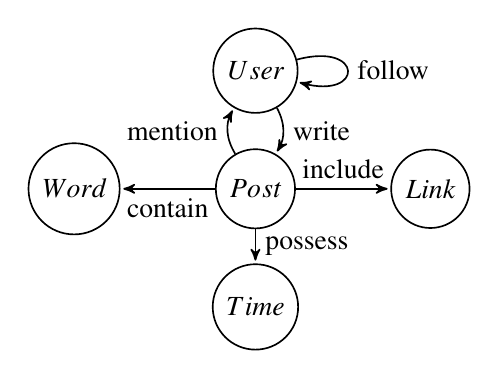
\begin{tikzpicture}[->,>=stealth',shorten >=1pt,auto,node distance=1.5cm,semithick]

  \node[state] (P)                    {$Post$};
  \node[state] (U) [above       of=P] {$User$};
  \node[state] (W) [left=1.2cm  of P] {$Word$};
  \node[state] (L) [right=1.2cm of P] {$Link$};
  \node[state] (T) [below       of=P] {$Time$};

  \path (U) edge [loop right] node {follow}  (U)
            edge [bend  left] node {write}   (P)
        (P) edge [bend  left] node {mention} (U)
            edge              node {include} (L)
            edge              node {contain} (W)
            edge              node {possess} (T);
\end{tikzpicture}
\caption{Schema of the Weibo network.}
\label{fig:schema}
\end{figure}

\begin{table}
\centering
\caption{Properties of the Weibo Sub-Network}
\label{table:stat}
\scriptsize
\begin{tabu} to \columnwidth {X[l] X[r] c X[l] X[r]}
\toprule
\multicolumn{2}{c}{\# Nodes} & & \multicolumn{2}{c}{\# Relations}\\
\cmidrule(l){1-2} \cmidrule{4-5}
User      & 3,000     & & follow        & 56,441 \\
Post      & 28,900    & & mention       & 6,662  \\
Word      & 1,177,343 & & contain       & 926,033\\
Link (URL)       & 7,524     & & include       & 7,521  \\
Time      & 24    & & write/possess & 28,900 \\
\bottomrule
\end{tabu}
\end{table}

\begin{table}
\centering
\caption{Similarity Meta-Paths Used for Feature Extraction}
\label{table:meta}
\scriptsize
\begin{tabu} to \columnwidth {X[c] X[l]}
\toprule
Meta-Path & Semantic Meaning \\
\midrule
$U\rightarrow~U\leftarrow~U$ & Common followee\\
$U\leftarrow~U\rightarrow~U$ & Common follower\\
$U\rightarrow~P\rightarrow~U\leftarrow~P\leftarrow~U$ & Common mentioned user\\
$U\rightarrow~P\rightarrow~W\leftarrow~P\leftarrow~U$ & Common word in posts\\
$U\rightarrow~P\rightarrow~L\leftarrow~P\leftarrow~U$ & Common referenced URL\\
$U\rightarrow~P\rightarrow~T\leftarrow~P\leftarrow~U$ & Common posting time\\
\bottomrule
\end{tabu}
\end{table}

\subsection{Experiments on real data}
We apply \npglm on real-world dataset to evaluate its effectiveness and compare its performance in predicting the time of link creation vis-\`a-vis different parametric models. 

\descr{Dataset.} We use a dynamic real-world dataset from \emph{Sina Weibo}, which is a Chinese microblogging social network. This dataset, provided by \cite{zhang2013}, is a heterogeneous social network whose meta structure is shown in Fig.~\ref{fig:schema}. It is composed of a static and a dynamic part: The static part describes the overal state of the network at the very first timestamp $t_0=$~September 27th 2012; and the dynamic part reflects the new following links along with their times occurred in a time window of 32 days, between September 28th to October 29th, 2012. Since the original dataset is too massive to process (having about 2 million users and 400 million following links), we confine the number of users to 3000 via random edge sampling with graph induction; a network sampling method which is shown to well preserve the topological structure of the original network \cite{ahmed2013}. The demographic statistics of the sampled network is presented in Table~\ref{table:stat}.

\begin{table*}[t]
\centering
\caption{Performance of Different Methods On the Weibo Dataset Under Different Measures}
\label{table:results}
%\tiny
\begin{tabu} to \textwidth {X[l] X[l] X[c] X[c] c X[c] X[c] X[c]}
\toprule
& 
& \multicolumn{2}{c}{Median Prediction Error} & & \multicolumn{3}{c}{Confidence Interval Prediction Accuracy (\%)}\\
\cmidrule(l){3-4} \cmidrule{6-8}
%\cmidrule(l){2-3} \cmidrule{5-7}
Dataset & 
Model & MAE & MRE & & 25\%-75\% & 20\%-80\% & 15\%-85\%\\
\midrule
\multirow{5}{*}{Sub-Network \#1} & 
\npglm & $\bm{10.59\pm0.18}$ & $\bm{4.41\pm0.50}$ & & $\bm{73.83\pm0.48}$ & $\bm{78.98\pm0.45}$ & $\bm{84.27\pm0.51}$\\
& 
\textsc{Exp-Glm} & $13.12\pm0.09$ & $6.79\pm0.05$ & & $47.78\pm0.19$ & $49.28\pm0.18$ & $51.03\pm0.24$\\
& 
\textsc{Ray-Glm} & $14.44\pm0.07$ & $9.51\pm0.07$ & & $48.84\pm0.10$ & $49.16\pm0.08$ & $49.55\pm0.07$\\
& 
\textsc{Pow-Glm} & $12.17\pm0.10$ & $5.77\pm0.11$ & & $51.19\pm0.31$ & $54.83\pm0.30$ & $61.83\pm0.51$\\
& 
\textsc{Gom-Glm} & $16.18\pm0.02$ & $11.07\pm0.04$ & & $43.73\pm0.17$ & $45.58\pm0.21$ & $46.66\pm0.15$\\
\midrule
\multirow{5}{*}{Sub-Network \#2} & 
\npglm & $\bm{10.19\pm0.10}$ & $\bm{4.43\pm0.07}$ & & $\bm{73.71\pm0.56}$ & $\bm{79.05\pm0.49}$ & $\bm{84.19\pm0.40}$\\
& \textsc{Exp-Glm} & $12.82\pm0.04$ & $6.67\pm0.05$ & & $47.88\pm0.22$ & $49.41\pm0.26$ & $51.48\pm0.27$\\
& \textsc{Ray-Glm} & $14.25\pm0.03$ & $9.38\pm0.04$ & & $48.84\pm0.11$ & $49.23\pm0.11$ & $49.67\pm0.12$\\
& \textsc{Pow-Glm} & $11.65\pm0.06$ & $5.50\pm0.08$ & & $52.07\pm0.25$ & $55.70\pm0.27$ & $62.51\pm0.35$\\
& \textsc{Gom-Glm} & $16.15\pm0.02$ & $11.03\pm0.05$ & & $44.05\pm0.23$ & $45.75\pm0.19$ & $46.67\pm0.15$\\
\midrule
\multirow{5}{*}{Sub-Network \#3} & 
\npglm & $\bm{10.34\pm0.12}$ & $\bm{4.41\pm0.02}$ & & $\bm{73.77\pm0.31}$ & $\bm{79.10\pm0.32}$ & $\bm{84.34\pm0.36}$\\
& \textsc{Exp-Glm} & $13.01\pm0.06$ & $6.73\pm0.02$ & & $47.66\pm0.17$ & $49.21\pm0.14$ & $51.02\pm0.13$\\
& \textsc{Ray-Glm} & $14.37\pm0.03$ & $9.45\pm0.03$ & & $48.81\pm0.08$ & $49.17\pm0.07$ & $49.58\pm0.08$\\
& \textsc{Pow-Glm} & $11.78\pm0.06$ & $5.53\pm0.06$ & & $51.64\pm0.17$ & $55.19\pm0.24$ & $62.15\pm0.22$\\
& \textsc{Gom-Glm} & $16.15\pm0.02$ & $11.04\pm0.02$ & & $43.88\pm0.25$ & $45.55\pm0.16$ & $46.55\pm0.16$\\
\bottomrule
\end{tabu}
\end{table*}

\descr{Experiment Setup.}
All pairs of users that establish a following relationship in the time window form our non-censored samples, whose number is about 57,000 pairs. We then randomly pick an equal number of user pairs who do not establish a following relationship, neither at the very first timestamp nor in the time window, as censored ones.

As the Weibo dataset is a heterogeneous social network, we use \emph{meta-paths} \cite{sun2011pathsim} to extract features for each pair of users. Regarding the network schema shown in Fig.~\ref{fig:schema}, we consider the symmetric similarity meta-paths presented in Table~\ref{table:meta}, where User, Post, Link, Time, and Word node types are denoted by $ U $, $ P $, $ L $, $ T $, and $ W $, respectively. For each sample pair of users, we apply the \emph{Path-Count} measure \cite{sun2011pathsim} on each meta-path to obtain a unique feature vector. Due to having different scales for different meta-paths, we normalize the obtained features using z-score.

To challenge the performance of the \npglm, we use ordinary generalized linear models with Exponential, Rayleigh, Power-Law, and Gompertz distributions, denoted as \textsc{Exp-Glm}, \textsc{Ray-Glm}, \textsc{Pow-Glm}, and \textsc{Gom-Glm}, respectively. We use 10-fold cross-validation and report the average results for all the experiments in this section.


\descr{Experiment Results.}
We evaluated the prediction performance of different methods using different sets of measures. First, for each test sample $x_{test}$, we considered the median of the distribution $f_T(t\mid~x_{test})$ as the predicted time for that sample and then compared it to the ground truth time $t_{test}$. Mean absolute error (MAE) and mean relative error (MRE) are used to measure the accuracy of the predicted values. Second, we inferred three different confidence intervals for each test sample and checked whether the ground truth time falls within these confidence intervals or not. Thereby, for each confidence interval, we calculated the percentage of the test samples for which their true times belong to that interval.

Table~\ref{table:results} presents the results obtained for each model under different settings. We can see that our \npglm method performs better than other ones under all measures. Comparing to its closest competitor, \textsc{Pow-Glm}, our method has reduced both MAE and MRE by about 13\% and 23\%, respectively. For confidence interval prediction, \npglm has gained a considerable accuracy in all three cases, which is far better than the other's. In 25\%-75\% confidence interval, \npglm has improved the accuracy by about 44\% relative to \textsc{Pow-Glm}. Under 20\%-80\% confidence interval, again an improvement of about 44\% has been achieved. Finally in 15\%-85\% confidence interval, \npglm can improve the accuracy of  \textsc{Pow-Glm} by about 36\%. These results confirms that the \npglm can better cope with the hidden underlying distribution of link creation time given the link features and it can well estimate this distribution and utilize it to do predictions.


\section{Related Works}\label{sec:related}
\newcommand{\etal}{\textit{et~al}.}

The problem of link prediction has been studied extensively in recent years and many approaches have been proposed to solve this problem \cite{wang2015link,wang2014review}.
Previous works on time-aware link prediction have mostly considered temporality in analyzing the long-term network trend over time \cite{dhote2013survey}. Authors in \cite{potgieter2009temporality} have shown that temporal metrics are an extremely valuable new contribution to link prediction, and should be used in future applications. 
%\cite{tylenda2009towards} incorporated temporal information available on evolving social networks for link prediction tasks and proposed a novel node-centric approach to the evaluation of link prediction. 
Dunlavy \etal{} focused on the problem of periodic temporal link prediction \cite{dunlavy2011temporal}. They focused on bipartite graphs that evolve over time and also considered weighted matrix that contained multilayer data and tensor-based methods for predicting future links.
Oyama \etal{} solved the problem of cross-temporal link prediction, in which the links among nodes in different time frames are inferred \cite{oyama2011cross}. They mapped data objects in different time frames into a common low-dimensional latent feature space, and identified the links on the basis of the distance between the data objects.
{\"O}zcan \etal{} proposed a novel link prediction method for evolving networks based on NARX neural network \cite{ozcan2016temporal}. They take the correlation between the quasi-local similarity measures and temporal evolutions of link occurrences information into account by using NARX for multivariate time series forecasting.
Yu \etal{} developed a novel temporal matrix factorization model to explicitly represent the network as a function of time \cite{yu2017temporally}. They provided results for link prediction as an specific example and showed that their model performs better than the state-of-the-art techniques.

The most relevant works to this study are available in \cite{hajibagheri2016leveraging, aggarwal2012dynamic, sett2017temporal, sun2012will}. The Authors in \cite{hajibagheri2016leveraging} approaches the problem of time series link prediction by extracting simple temporal features from the time series, such as mean, (weighted) moving average, and exponential smoothing besides some topological features like common neighbor and adamic-adar. But their method is designed for homogeneous networks and fail to consider the heterogeneity of the modern networks. Aggarwal \etal{} \cite{aggarwal2012dynamic} tackle the link prediction problem in both dynamic and heterogeneous information networks using a dynamic clustering approach alongside with content-based and structural models. However they aim to solve the conventional link prediction problem, not the continuous-time relationship prediction problem studied in this paper. In \cite{sett2017temporal}, the authors proposed a feature set, called TMLP, well suited for link prediction in dynamic and heterogeneous information networks. Although their proposed feature set cope with both dynamicity and heterogeneity of the network, it cannot be extended for the generalized problem of relationship prediction and is only designed for solving the simpler link prediction problem.

Most of the aforementioned works answered the question of \emph{whether} a link will appear in the network. To the best of our knowledge, the only work that has focused on the continuous-time relationship prediction problem is proposed by Sun \etal{} \cite{sun2012will}, in which a generalized linear model based framework is suggested to model the relationship building time. They consider the building time of links as independent random variables coming from a pre-specified distribution and model the expectation as a function of a linear predictor of the extracted topological features. A shortcoming of this model is that we need to exactly specify the underlying distribution of times. We came over this problem by learning the distribution from the data using a non-parametric solution. Furthermore, we considered the temporal dynamics of the network which has been entirely ignored in their work.

\begin{table*}[t]
	\scriptsize
	\centering
	\caption{Performance Comparison of Different Methods Under Different Lengths for Feature Extraction Window when $\Omega=6$}
	\label{table:results2}
	%\tiny
	\begin{tabu} to \textwidth {X[l] c l X[c] X[c] c X[c] X[c] c X[c] X[c]}
		\toprule
		& & 
		& \multicolumn{2}{c}{$\Phi=5$} & & \multicolumn{2}{c}{$\Phi=10$} & & \multicolumn{2}{c}{$\Phi=15$}\\
		\cmidrule(l){4-5} \cmidrule{7-8} \cmidrule{10-11}
		%\cmidrule(l){2-3} \cmidrule{5-7}
		Dataset & Feature &
		Model & MAE & MRE & & MAE & MRE & & MAE & MRE\\
		\midrule
		\multirow{8}{*}{dblp-db}
		& \multirow{4}{*}{\rotatebox{90}{Dynamic}}
		& 			  \npglm & $\bm{0.78\pm0.01}$ & $\bm{0.37\pm0.01}$ & & $\bm{0.76\pm0.05}$ & $\bm{0.34\pm0.03}$ & & $\bm{0.62\pm0.07}$ & $\bm{0.35\pm0.03}$ \\
		& & \textsc{Exp-Glm} & $0.83\pm0.02$ & $0.41\pm0.05$ & & $0.83\pm0.09$ & $0.43\pm0.06$ & & $0.76\pm0.07$ & $0.40\pm0.03$ \\
		& & \textsc{Ray-Glm} & $1.65\pm0.08$ & $1.00\pm0.03$ & & $1.90\pm0.06$ & $1.00\pm0.09$ & & $1.84\pm0.04$ & $1.00\pm0.02$ \\
		& & \textsc{Gom-Glm} & $2.05\pm0.06$ & $1.12\pm0.06$ & & $1.89\pm0.07$ & $1.23\pm0.02$ & & $1.95\pm0.01$ & $1.17\pm0.08$ \\
		
		\cmidrule{2-11}                                                                            
		& \multirow{4}{*}{\rotatebox{90}{Static}}                                                  
		& 			  \npglm & $0.86\pm0.02$ & $0.44\pm0.01$ & & $0.85\pm0.03$ & $0.44\pm0.02$ & & $0.81\pm0.05$ & $0.41\pm0.02$ \\
		& & \textsc{Exp-Glm} & $0.94\pm0.03$ & $0.50\pm0.02$ & & $0.93\pm0.03$ & $0.51\pm0.02$ & & $0.93\pm0.04$ & $0.51\pm0.03$ \\
		& & \textsc{Ray-Glm} & $2.17\pm0.05$ & $1.29\pm0.04$ & & $2.16\pm0.04$ & $1.29\pm0.03$ & & $2.12\pm0.07$ & $1.28\pm0.05$ \\
		& & \textsc{Gom-Glm} & $2.28\pm0.03$ & $1.35\pm0.02$ & & $2.28\pm0.06$ & $1.36\pm0.04$ & & $2.22\pm0.08$ & $1.34\pm0.07$ \\
		
		\midrule                                                                                   
		\multirow{8}{*}{dblp-th}                                                                   
		& \multirow{4}{*}{\rotatebox{90}{Dynamic}}                                                 
		& 			  \npglm & $\bm{0.77\pm0.01}$ & $\bm{0.40\pm0.01}$ & & $\bm{0.75\pm0.09}$ & $\bm{0.36\pm0.02}$ & & $\bm{0.70\pm0.04}$ & $\bm{0.36\pm0.09}$ \\
		& & \textsc{Exp-Glm} & $0.85\pm0.06$ & $0.40\pm0.09$ & & $0.75\pm0.09$ & $0.43\pm0.06$ & & $0.75\pm0.08$ & $0.47\pm0.02$ \\
		& & \textsc{Ray-Glm} & $1.77\pm0.05$ & $1.15\pm0.09$ & & $1.83\pm0.06$ & $1.11\pm0.02$ & & $1.95\pm0.08$ & $1.10\pm0.06$ \\
		& & \textsc{Gom-Glm} & $2.10\pm0.06$ & $1.07\pm0.03$ & & $1.88\pm0.05$ & $1.23\pm0.02$ & & $1.76\pm0.04$ & $1.08\pm0.05$ \\
		
		\cmidrule{2-11}                                                                            
		& \multirow{4}{*}{\rotatebox{90}{Static}}                                                  
		& 			  \npglm & $0.90\pm0.03$ & $0.46\pm0.01$ & & $0.89\pm0.04$ & $0.45\pm0.01$ & & $0.85\pm0.04$ & $0.43\pm0.03$ \\
		& & \textsc{Exp-Glm} & $0.98\pm0.03$ & $0.52\pm0.03$ & & $0.97\pm0.03$ & $0.53\pm0.03$ & & $0.98\pm0.04$ & $0.54\pm0.03$ \\
		& & \textsc{Ray-Glm} & $2.33\pm0.07$ & $1.32\pm0.04$ & & $2.29\pm0.04$ & $1.36\pm0.04$ & & $2.21\pm0.12$ & $1.34\pm0.08$ \\
		& & \textsc{Gom-Glm} & $2.42\pm0.04$ & $1.41\pm0.06$ & & $2.40\pm0.08$ & $1.41\pm0.06$ & & $2.31\pm0.08$ & $1.40\pm0.07$ \\
		
		\bottomrule
	\end{tabu}
\end{table*}
\section{Conclusion}\label{sec:conclusion}
In this paper, we studied the problem of temporal link prediction and proposed a probabilistic non-parametric method, \npglm, to predict the time of link creation in social networks. Our method does not impose any significant assumption on the underlying distribution of the link's advent time given its features, but tries to infer it from the data via a non-parametric approach. Extensive experiments conducted on both synthetic dataset and real-world data from Weibo social network demonstrated the correctness of our method and its effectiveness in predicting the formation time of links.\\
%\section*{Acknowledgements}
We would like to thank anonymous reviewers for their comments and feedbacks on this paper. We also appreciate ICT Innovation Center of Sharif University of Technology for their financial support.
%\input{appendix}

\bibliographystyle{IEEEtran}
\balance
\bibliography{IEEEabrv,IEEEexample}

\end{document}
